\documentclass[margin=2mm]{standalone}
\usepackage{tikz}
\usepackage{pgfplots}
\usepgfplotslibrary{colorbrewer}
\usetikzlibrary{positioning}
\usetikzlibrary{arrows}

\definecolor{s1}{RGB}{204, 76, 2}

\begin{document}
  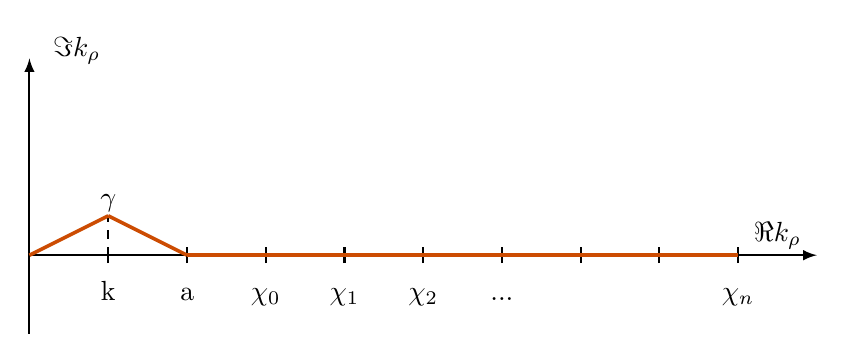
\begin{tikzpicture}
    \tikzstyle{bplus}=[rectangle split, rectangle split horizontal,
    rectangle split ignore empty parts, rectangle split part align=base,draw]

    % Draw coordinate system
    % x-axis
    \draw [line width=0.25mm, arrows={-latex}, color=black] (0, 0) -- (10, 0);
    % y-axis
    \draw [line width=0.25mm, arrows={-latex}, color=black] (0, -1) -- (0, 2.5);
    % x-axis label
    \node at (9.5, 0.25) {$\Re {k_{\rho}}$};
    % y-axis label
    \node at (0.6, 2.6) {$\Im {k_{\rho}}$};

    % Tick label
    \node  [anchor=mid] at (1, -.5)  {k};
    % Tick
    \draw[thick] (1, -.1) -- (1, .1);
    % Tick label
    \node  [anchor=mid] at (2, -.5)  {a};
    % Tick
    \draw[thick] (2, -.1) -- (2, .1);
    % Tick label
    \node [anchor=mid] at (3, -.5)  {$\chi_0$};
    % Tick
    \draw[thick] (3, -.1) -- (3, .1);
    % Tick label
    \node [anchor=mid] at (4, -.5)  {$\chi_1$};
    % Tick
    \draw[thick] (4, -.1) -- (4, .1);
    % Tick label
    \node [anchor=mid] at (5, -.5)  {$\chi_2$};
    % Tick
    \draw[thick] (5, -.1) -- (5, .1);
    % Tick label
    \node [anchor=mid] at (6, -.5)  {...};
    % Tick
    \draw[thick] (6, -.1) -- (6, .1);
    % Tick
    \draw[thick] (7, -.1) -- (7, .1);
    % Tick
    \draw[thick] (8, -.1) -- (8, .1);
    % Tick label
    \node [anchor=mid] at (9, -.5)  {$\chi_n$};
    % Tick
    \draw[thick] (9, -.1) -- (9, .1);

    % Draw the indented value
    \draw [line width=0.25mm, color=black, dashed] (1, 0) -- (1, .5);

    % Draw the integration path
    \draw [line width=0.45mm, color=s1] (0, 0) -- (1, .5);
    \node [anchor=mid] at (1, .7)  {$\gamma$};
    \draw [line width=0.45mm, color=s1] (1, .5) -- (2, 0);
    \draw [line width=0.45mm, color=s1] (2, 0) -- (9, 0);


  \end{tikzpicture}
\end{document}
